% Options for packages loaded elsewhere
\PassOptionsToPackage{unicode}{hyperref}
\PassOptionsToPackage{hyphens}{url}
%
\documentclass[
]{article}
\usepackage{amsmath,amssymb}
\usepackage{lmodern}
\usepackage{iftex}
\ifPDFTeX
  \usepackage[T1]{fontenc}
  \usepackage[utf8]{inputenc}
  \usepackage{textcomp} % provide euro and other symbols
\else % if luatex or xetex
  \usepackage{unicode-math}
  \defaultfontfeatures{Scale=MatchLowercase}
  \defaultfontfeatures[\rmfamily]{Ligatures=TeX,Scale=1}
\fi
% Use upquote if available, for straight quotes in verbatim environments
\IfFileExists{upquote.sty}{\usepackage{upquote}}{}
\IfFileExists{microtype.sty}{% use microtype if available
  \usepackage[]{microtype}
  \UseMicrotypeSet[protrusion]{basicmath} % disable protrusion for tt fonts
}{}
\makeatletter
\@ifundefined{KOMAClassName}{% if non-KOMA class
  \IfFileExists{parskip.sty}{%
    \usepackage{parskip}
  }{% else
    \setlength{\parindent}{0pt}
    \setlength{\parskip}{6pt plus 2pt minus 1pt}}
}{% if KOMA class
  \KOMAoptions{parskip=half}}
\makeatother
\usepackage{xcolor}
\IfFileExists{xurl.sty}{\usepackage{xurl}}{} % add URL line breaks if available
\IfFileExists{bookmark.sty}{\usepackage{bookmark}}{\usepackage{hyperref}}
\hypersetup{
  pdftitle={California Collaborative Fisheries Research Program},
  pdfauthor={Compiled by Melissa H. Monk (SWFSC)},
  hidelinks,
  pdfcreator={LaTeX via pandoc}}
\urlstyle{same} % disable monospaced font for URLs
\usepackage[margin=1in]{geometry}
\usepackage{longtable,booktabs,array}
\usepackage{calc} % for calculating minipage widths
% Correct order of tables after \paragraph or \subparagraph
\usepackage{etoolbox}
\makeatletter
\patchcmd\longtable{\par}{\if@noskipsec\mbox{}\fi\par}{}{}
\makeatother
% Allow footnotes in longtable head/foot
\IfFileExists{footnotehyper.sty}{\usepackage{footnotehyper}}{\usepackage{footnote}}
\makesavenoteenv{longtable}
\usepackage{graphicx}
\makeatletter
\def\maxwidth{\ifdim\Gin@nat@width>\linewidth\linewidth\else\Gin@nat@width\fi}
\def\maxheight{\ifdim\Gin@nat@height>\textheight\textheight\else\Gin@nat@height\fi}
\makeatother
% Scale images if necessary, so that they will not overflow the page
% margins by default, and it is still possible to overwrite the defaults
% using explicit options in \includegraphics[width, height, ...]{}
\setkeys{Gin}{width=\maxwidth,height=\maxheight,keepaspectratio}
% Set default figure placement to htbp
\makeatletter
\def\fps@figure{htbp}
\makeatother
\setlength{\emergencystretch}{3em} % prevent overfull lines
\providecommand{\tightlist}{%
  \setlength{\itemsep}{0pt}\setlength{\parskip}{0pt}}
\setcounter{secnumdepth}{5}
\usepackage{booktabs}
\usepackage{longtable}
\usepackage{array}
\usepackage{multirow}
\usepackage{wrapfig}
\usepackage{float}
\usepackage{colortbl}
\usepackage{pdflscape}
\usepackage{tabu}
\usepackage{threeparttable}
\usepackage[normalem]{ulem}
\usepackage{makecell}
\usepackage{xcolor}
\usepackage{placeins}
\usepackage{booktabs}
\usepackage{longtable}
\usepackage{array}
\usepackage{multirow}
\usepackage{wrapfig}
\usepackage{float}
\usepackage{colortbl}
\usepackage{pdflscape}
\usepackage{tabu}
\usepackage{threeparttable}
\usepackage{threeparttablex}
\usepackage[normalem]{ulem}
\usepackage{makecell}
\usepackage{xcolor}
\ifLuaTeX
  \usepackage{selnolig}  % disable illegal ligatures
\fi

\title{California Collaborative Fisheries Research Program}
\usepackage{etoolbox}
\makeatletter
\providecommand{\subtitle}[1]{% add subtitle to \maketitle
  \apptocmd{\@title}{\par {\large #1 \par}}{}{}
}
\makeatother
\subtitle{Data availability for stock assessments}
\author{Compiled by Melissa H. Monk (SWFSC)}
\date{May 09, 2022}

\begin{document}
\maketitle

\newcommand\CapeM{$40^\circ 10^\prime N$}

\hypertarget{summary}{%
\section{Summary}\label{summary}}

This document summarizes the data from the California Collaborative
Fisheries Research Program (CCFRP) as well as the available data for the four
species proposed for stock assessments in 2023, including black rockfish (\emph{Sebastes melanops}),
copper rockfish (\emph{S. caurinus}), quillback rockfish (\emph{S. maliger}), and
yellowtail rockfish (\emph{S. flavidus}). Preliminary analyses suggest the following
data availability to inform stock assessments for each species:

\textbf{Black rockfish}: There are enough data to consider an index of abundance and also
include ages in the assessment model.

\textbf{Copper rockfish}: There are enough data north of Point Conception to consider an
index of abundance. The two MPAs south of Point Conception with consistent encounters
of copper rockfish cover a very small fraction of the available habitat and were not
included in the original sampling design. There are enough age data available north
of Point Conception for inclusion in an assessment model. Otoliths will be
collected south of Point Conception in 2022.

\textbf{Quillback rockfish}: There is only one MPA monitored north of the $40^\circ 10^\prime N$ management
boundary in California that was not part of the original sampling design and hence
does not have a long time series. It is not likely that robust index can be developed
from the sparse data separately north and south of $40^\circ 10^\prime N$. An exploration of an index
could be considered if California is modeled as one area. Age data are available t
hat could inform growth external to the assessment model.

\textbf{Yellowtail rockfish}: There are enough data to consider an index of abundance north of
Point Conception for yellowtail rockfish as well as include age data from the otoliths
within the assessment model.

\hypertarget{survey-background}{%
\section{Survey Background}\label{survey-background}}

The 1999 Marine Life Protection Act resulted in the creation of a network of
Marine Protected Areas (MPAs) along California's coast. The state of California
designated both State Marine Reserves (SMRs) and State Marine Recreational
Management areas (SMCAs). The SMRs prohibit all recreational and commercial take
and SMCAs allow some recreational and/or commercial take that varies by SMCA.
A number of MPAs consist of an SMR adjacent to an SMCA, of which the SMR is closer to shore.
The California Collaborative Fisheries Research Program,
\href{https://www.mlml.calstate.edu/ccfrp/}{CCFRP},
is a fishery-independent hook-and-line survey designed to monitor nearshore fish
populations at a series of sampling locations both inside and adjacent to
California's network of MPAs.

The CCFRP survey began in 2007 with Cal Poly and Moss Landing Marine Labs
in collaboration with NMFS scientists and the fishing community. The core
area of the survey includes Año Nuevo SMR and Point Lobos SMR sampled by
San Jose State University Moss Landing Marine Lab, and Point Buchon SMR
and Piedras Blancas SMR sampled by California Polytechnic University
San Luis Obispo (Figure \ref{fig:fig-mpa-map}). In 2017, CCFRP expanded within
California to include four additional partners, Cal Poly Humboldt (formerly Humboldt State
University), University of California Davis' Bodega Marine Lab, University
of California Santa Barbara, and the Scripps Institute of Oceanography.
The CCFRP now monitors 12 MPA and reference area pairs (Table \ref{tab:monitoring}).
Cal Poly Humboldt samples the furthest north sites, which are south of Cape
Mendocino, but north of the management line at $40^\circ 10^\prime N$. There are three nearshore
SMCAs north of Cape Mendocino that
were not selected for CCFRP monitoring due to historical sampling the tiers
assigned to the SMRs by CDFW. The COVID-19 pandemic also affected the
survey effort, but all partners were able to conduct sampling in 2000 and 2001.

The CCFRP survey design is consistent across all partners. Each MPA and reference
area consists of a number of 500 x 500 m cells that were selected because the contained
appropriate rockfish habitat. The survey was designed as a capture
and release survey, with a sub-study tag/recapture program. Therefore, CCFRP restricts
sampling areas to depths shallower than approximately 120 feet in order to reduce
potential effects of barotrauma. On any given survey
day site cells are randomly selected within a stratum (MPA and/or reference cells).
Commercial passenger fishing vessels (CPFVs) are chartered for the survey and
the captain is allowed to search within the cell for a fishing location.
Due to the nature of the fishery in northern California, Cal Poly Humboldt conducts
sampling aboard 6-pack vessels, and therefore fishes for fewer total angler hours per
year compared to the other partners (Tables \ref{tab:anghrs} and \ref{tab:fishingdrops}). During
a sampling event, each cell is fished for a total of 30-45 minutes by volunteer
anglers. Volunteer anglers are allowed to reel up their lines at any time during a
fishing drop if they think they've hooked fish. Anglers can then re-bait and
continue fishing until the the drop is complete. Each fish encountered
can be linked back to an angler. Each anglers fishes one line, with two hooks.
The jig and bait is assigned to each angler, but an angler may fish with a personal
fishing rod.

All fish encountered are measured to the nearest centimeter (fork length), and the
majority of fish are released or descended to depth.
A total of 58498 fish were tagged
since 2007, and recapture data are available from each partner. Starting in 2017,
at the request of Melissa Monk (NMFS SWFSC), a fraction of the fish encountered
in the reference cells have been retained to collect otoliths and fin clips that
provide needed biological information for nearshore species. In 2022, the goal
is to increase biological collections for commonly encountered species for use
in the 2023 stock assessments.

\hypertarget{available-data-for-indices}{%
\section{Available Data for Indices}\label{available-data-for-indices}}

From 2007-2021 a total of 698 fishing trips
were taken, consisting of 9634 fishing drops. When the CCFRP
expanded in 2017, some MPAs/sites were fished in only one or two years during an
exploratory phase. These included Laguna Beach, the southeast Farallon Islands,
Point Conception and Trinidad, which were excluded from this summary since we
would not include them in a stock assessment.
Fishing drops that drifted outside a cell were also excluded. These site filter
result in an available 7910. The final filter removed
drifts within a cell that were not fished for at least ten minutes within a sampling
occasion, resulting in a total of 7889 fishing
drops available for analyses for stock assessments. The total nubmer of fish
encountered by CCFRP partner and the percent of positive drops by species and MPA
can be found in Tables \ref{tab:totalfishbygroup} - \ref{tab:percentpos}.

\hypertarget{available-lengths-and-otoliths}{%
\section{Available Lengths and Otoliths}\label{available-lengths-and-otoliths}}

The CCFRP measures every fish to the nearest centimeter and distributions of the
lengths inside and outside the MPAs by MPA and species are in Figures
\ref{fig:lengths-1} - \ref{fig:lengths-4}. Length data were
filtered to the drifts included in the final data set. Any species and MPA combination
with fewer than 20 observed fish in an MPA or reference area over the entirety
of the program were removed from the length plots.

The total number of fish retained by university partner can be found in Table
\ref{tab:otoliths}. This represents that maximum number of available otoliths,
which will be verified once the stock assessments for 2023 are verified. The
rule of thumb for including conditional age-at-length samples is a minimum of 30
available fish in a year/fleet stratum. Given this, there are likely not enough
fish from Bodega or Cal Poly for any species.

\FloatBarrier
\newpage

\hypertarget{tables}{%
\section{Tables}\label{tables}}

\FloatBarrier

\begin{table}

\caption{\label{tab:monitoring}Monitoring groups and the associated MPAs they sample. The abbreviated names will be 
  used throughout most of the tables in this document}
\centering
\begin{tabular}[t]{lll}
\toprule
Monitoring Group & Abbreviated Name & MPA\\
\midrule
\cellcolor{gray!6}{Cal Poly Humboldt} & \cellcolor{gray!6}{Humboldt} & \cellcolor{gray!6}{South Cape Mendocino}\\
Cal Poly Humboldt & Humboldt & Ten Mile\\
\cellcolor{gray!6}{Bodega Marine Lab} & \cellcolor{gray!6}{Bodega} & \cellcolor{gray!6}{Stewarts Point}\\
Bodega Marine Lab & Bodega & Bodega Head\\
\cellcolor{gray!6}{Moss Landing Marine Lab} & \cellcolor{gray!6}{Moss Landing} & \cellcolor{gray!6}{Ano Nuevo}\\
\addlinespace
Moss Landing Marine Lab & Moss Landing & Point Lobos\\
\cellcolor{gray!6}{Cal Poly SLO} & \cellcolor{gray!6}{Cal Poly} & \cellcolor{gray!6}{Piedras Blancas}\\
Cal Poly SLO & Cal Poly & Point Buchon\\
\cellcolor{gray!6}{UC Santa Barbara} & \cellcolor{gray!6}{UCSB} & \cellcolor{gray!6}{Carrington Point}\\
UC Santa Barbara & UCSB & Anacapa Island\\
\addlinespace
\cellcolor{gray!6}{Scripps Institute Ocean.} & \cellcolor{gray!6}{Scripps} & \cellcolor{gray!6}{Swamis}\\
Scripps Institute Ocean. & Scripps & South La Jolla\\
\bottomrule
\end{tabular}
\end{table}

\begin{table}

\caption{\label{tab:anghrs}Total angler hours by institution summed across all active years.}
\centering
\begin{tabular}[t]{r>{\raggedleft\arraybackslash}p{6em}>{\raggedleft\arraybackslash}p{6em}>{\raggedleft\arraybackslash}p{6em}>{\raggedleft\arraybackslash}p{6em}>{\raggedleft\arraybackslash}p{6em}>{\raggedleft\arraybackslash}p{6em}}
\toprule
YEAR & Humboldt & Bodega & Moss Landing & Cal Poly & UCSB & Scripps\\
\midrule
\cellcolor{gray!6}{2007} & \cellcolor{gray!6}{0} & \cellcolor{gray!6}{0} & \cellcolor{gray!6}{450} & \cellcolor{gray!6}{277} & \cellcolor{gray!6}{0} & \cellcolor{gray!6}{0}\\
2008 & 0 & 0 & 639 & 455 & 0 & 0\\
\cellcolor{gray!6}{2009} & \cellcolor{gray!6}{0} & \cellcolor{gray!6}{0} & \cellcolor{gray!6}{343} & \cellcolor{gray!6}{339} & \cellcolor{gray!6}{0} & \cellcolor{gray!6}{0}\\
2010 & 0 & 0 & 406 & 440 & 0 & 0\\
\cellcolor{gray!6}{2011} & \cellcolor{gray!6}{0} & \cellcolor{gray!6}{0} & \cellcolor{gray!6}{459} & \cellcolor{gray!6}{393} & \cellcolor{gray!6}{0} & \cellcolor{gray!6}{0}\\
\addlinespace
2012 & 0 & 0 & 526 & 422 & 0 & 0\\
\cellcolor{gray!6}{2013} & \cellcolor{gray!6}{0} & \cellcolor{gray!6}{0} & \cellcolor{gray!6}{484} & \cellcolor{gray!6}{376} & \cellcolor{gray!6}{0} & \cellcolor{gray!6}{0}\\
2014 & 0 & 0 & 522 & 473 & 0 & 0\\
\cellcolor{gray!6}{2015} & \cellcolor{gray!6}{0} & \cellcolor{gray!6}{0} & \cellcolor{gray!6}{264} & \cellcolor{gray!6}{272} & \cellcolor{gray!6}{0} & \cellcolor{gray!6}{0}\\
2016 & 0 & 0 & 524 & 532 & 0 & 0\\
\addlinespace
\cellcolor{gray!6}{2017} & \cellcolor{gray!6}{157} & \cellcolor{gray!6}{92} & \cellcolor{gray!6}{383} & \cellcolor{gray!6}{507} & \cellcolor{gray!6}{137} & \cellcolor{gray!6}{127}\\
2018 & 136 & 353 & 330 & 373 & 230 & 186\\
\cellcolor{gray!6}{2019} & \cellcolor{gray!6}{132} & \cellcolor{gray!6}{403} & \cellcolor{gray!6}{365} & \cellcolor{gray!6}{340} & \cellcolor{gray!6}{222} & \cellcolor{gray!6}{240}\\
2020 & 103 & 143 & 198 & 222 & 227 & 105\\
\cellcolor{gray!6}{2021} & \cellcolor{gray!6}{127} & \cellcolor{gray!6}{219} & \cellcolor{gray!6}{305} & \cellcolor{gray!6}{246} & \cellcolor{gray!6}{271} & \cellcolor{gray!6}{109}\\
\bottomrule
\end{tabular}
\end{table}

\begin{landscape}\begin{table}

\caption{\label{tab:fishingdrops}Total number of fishing drops by year at each monitored site in the reference areas and inside the MPAs, in parentheses.}
\centering
\resizebox{\linewidth}{!}{
\begin{tabular}[t]{r>{\raggedright\arraybackslash}p{1.7cm}>{\raggedright\arraybackslash}p{1.5cm}>{\raggedright\arraybackslash}p{1.5cm}>{\raggedright\arraybackslash}p{1.5cm}>{\raggedright\arraybackslash}p{1.5cm}>{\raggedright\arraybackslash}p{1.5cm}>{\raggedright\arraybackslash}p{1.5cm}>{\raggedright\arraybackslash}p{1.5cm}>{\raggedright\arraybackslash}p{1.5cm}>{\raggedright\arraybackslash}p{1.5cm}>{\raggedright\arraybackslash}p{1.5cm}l}
\toprule
\multicolumn{1}{c}{ } & \multicolumn{2}{c}{Cal Poly Humboldt} & \multicolumn{2}{c}{Bodega Marine Lab} & \multicolumn{2}{c}{Moss Landing} & \multicolumn{2}{c}{Cal Poly SLO} & \multicolumn{2}{c}{UC Santa Barbara} & \multicolumn{2}{c}{Scripps} \\
\cmidrule(l{3pt}r{3pt}){2-3} \cmidrule(l{3pt}r{3pt}){4-5} \cmidrule(l{3pt}r{3pt}){6-7} \cmidrule(l{3pt}r{3pt}){8-9} \cmidrule(l{3pt}r{3pt}){10-11} \cmidrule(l{3pt}r{3pt}){12-13}
YEAR & South Cape Mendocino & Ten Mile & Stewarts Point & Bodega Head & Ano Nuevo & Point Lobos & Piedras Blancas & Point Buchon & Carrington Point & Anacapa Island & Swamis & South La Jolla\\
\midrule
\cellcolor{gray!6}{2007} & \cellcolor{gray!6}{-} & \cellcolor{gray!6}{-} & \cellcolor{gray!6}{-} & \cellcolor{gray!6}{-} & \cellcolor{gray!6}{125(72)} & \cellcolor{gray!6}{70(93)} & \cellcolor{gray!6}{-} & \cellcolor{gray!6}{64(71)} & \cellcolor{gray!6}{-} & \cellcolor{gray!6}{-} & \cellcolor{gray!6}{-} & \cellcolor{gray!6}{-}\\
2008 & - & - & - & - & 90(101) & 74(82) & 30(45) & 62(65) & - & - & - & -\\
\cellcolor{gray!6}{2009} & \cellcolor{gray!6}{-} & \cellcolor{gray!6}{-} & \cellcolor{gray!6}{-} & \cellcolor{gray!6}{-} & \cellcolor{gray!6}{78(45)} & \cellcolor{gray!6}{38(45)} & \cellcolor{gray!6}{38(35)} & \cellcolor{gray!6}{46(40)} & \cellcolor{gray!6}{-} & \cellcolor{gray!6}{-} & \cellcolor{gray!6}{-} & \cellcolor{gray!6}{-}\\
2010 & - & - & - & - & 76(80) & 45(48) & 44(39) & 44(46) & - & - & - & -\\
\cellcolor{gray!6}{2011} & \cellcolor{gray!6}{-} & \cellcolor{gray!6}{-} & \cellcolor{gray!6}{-} & \cellcolor{gray!6}{-} & \cellcolor{gray!6}{54(58)} & \cellcolor{gray!6}{40(49)} & \cellcolor{gray!6}{42(36)} & \cellcolor{gray!6}{44(42)} & \cellcolor{gray!6}{-} & \cellcolor{gray!6}{-} & \cellcolor{gray!6}{-} & \cellcolor{gray!6}{-}\\
\addlinespace
2012 & - & - & - & - & 63(62) & 50(48) & 40(39) & 45(43) & - & - & - & -\\
\cellcolor{gray!6}{2013} & \cellcolor{gray!6}{-} & \cellcolor{gray!6}{-} & \cellcolor{gray!6}{-} & \cellcolor{gray!6}{-} & \cellcolor{gray!6}{66(71)} & \cellcolor{gray!6}{58(53)} & \cellcolor{gray!6}{41(38)} & \cellcolor{gray!6}{40(52)} & \cellcolor{gray!6}{-} & \cellcolor{gray!6}{-} & \cellcolor{gray!6}{-} & \cellcolor{gray!6}{-}\\
2014 & - & - & - & - & 66(77) & 57(55) & 46(46) & 50(44) & - & - & - & -\\
\cellcolor{gray!6}{2015} & \cellcolor{gray!6}{-} & \cellcolor{gray!6}{-} & \cellcolor{gray!6}{-} & \cellcolor{gray!6}{-} & \cellcolor{gray!6}{37(39)} & \cellcolor{gray!6}{24(27)} & \cellcolor{gray!6}{-} & \cellcolor{gray!6}{49(49)} & \cellcolor{gray!6}{-} & \cellcolor{gray!6}{-} & \cellcolor{gray!6}{-} & \cellcolor{gray!6}{-}\\
2016 & - & - & - & - & 66(57) & 47(50) & 47(57) & 48(49) & - & - & - & -\\
\addlinespace
\cellcolor{gray!6}{2017} & \cellcolor{gray!6}{38(34)} & \cellcolor{gray!6}{44(43)} & \cellcolor{gray!6}{13(9)} & \cellcolor{gray!6}{15(14)} & \cellcolor{gray!6}{59(48)} & \cellcolor{gray!6}{35(37)} & \cellcolor{gray!6}{44(46)} & \cellcolor{gray!6}{48(48)} & \cellcolor{gray!6}{17(17)} & \cellcolor{gray!6}{14(7)} & \cellcolor{gray!6}{9(7)} & \cellcolor{gray!6}{10(21)}\\
2018 & 36(33) & 34(35) & 47(54) & 36(34) & 54(50) & 31(34) & 34(35) & 36(34) & 29(26) & 21(16) & 16(6) & 22(28)\\
\cellcolor{gray!6}{2019} & \cellcolor{gray!6}{34(35)} & \cellcolor{gray!6}{32(36)} & \cellcolor{gray!6}{50(60)} & \cellcolor{gray!6}{41(40)} & \cellcolor{gray!6}{47(46)} & \cellcolor{gray!6}{35(38)} & \cellcolor{gray!6}{34(32)} & \cellcolor{gray!6}{36(39)} & \cellcolor{gray!6}{25(27)} & \cellcolor{gray!6}{19(12)} & \cellcolor{gray!6}{12(13)} & \cellcolor{gray!6}{24(23)}\\
2020 & 30(36) & 34(35) & 26(46) & 43(39) & 59(51) & 34(44) & 35(30) & 35(35) & 36(36) & 23(11) & 9(10) & 26(33)\\
\cellcolor{gray!6}{2021} & \cellcolor{gray!6}{37(35)} & \cellcolor{gray!6}{35(33)} & \cellcolor{gray!6}{28(41)} & \cellcolor{gray!6}{38(31)} & \cellcolor{gray!6}{51(46)} & \cellcolor{gray!6}{38(41)} & \cellcolor{gray!6}{32(36)} & \cellcolor{gray!6}{33(35)} & \cellcolor{gray!6}{31(35)} & \cellcolor{gray!6}{20(12)} & \cellcolor{gray!6}{6(8)} & \cellcolor{gray!6}{23(28)}\\
\bottomrule
\end{tabular}}
\end{table}
\end{landscape}

\FloatBarrier
\newpage

\FloatBarrier

\begin{table}

\caption{\label{tab:totalfishbygroup}Total number of fish encountered by each monitoring group.}
\centering
\begin{tabular}[t]{lrrrrrr}
\toprule
Common.Name & Humboldt & Bodega & Moss Landing & Cal Poly & UCSB & Scripps\\
\midrule
\cellcolor{gray!6}{Black Rockfish} & \cellcolor{gray!6}{1296} & \cellcolor{gray!6}{1488} & \cellcolor{gray!6}{13272} & \cellcolor{gray!6}{1744} & \cellcolor{gray!6}{2} & \cellcolor{gray!6}{0}\\
Copper Rockfish & 365 & 509 & 901 & 1008 & 2352 & 46\\
\cellcolor{gray!6}{Quillback Rockfish} & \cellcolor{gray!6}{220} & \cellcolor{gray!6}{39} & \cellcolor{gray!6}{1} & \cellcolor{gray!6}{1} & \cellcolor{gray!6}{0} & \cellcolor{gray!6}{0}\\
Yellowtail Rockfish & 482 & 979 & 1828 & 1029 & 6 & 0\\
\bottomrule
\end{tabular}
\end{table}

\begin{landscape}\begin{table}

\caption{\label{tab:percentpos}Percent of drifts with encounters of Black Rockfish in each at each monitoring location and yerar.}
\centering
\begin{tabular}[t]{r>{\raggedright\arraybackslash}p{1.7cm}>{\raggedright\arraybackslash}p{1.2cm}>{\raggedright\arraybackslash}p{1.2cm}>{\raggedright\arraybackslash}p{1.2cm}>{\raggedright\arraybackslash}p{1.2cm}>{\raggedright\arraybackslash}p{1.2cm}>{\raggedright\arraybackslash}p{1.2cm}>{\raggedright\arraybackslash}p{1.2cm}>{\raggedright\arraybackslash}p{1.7cm}>{\raggedright\arraybackslash}p{1.2cm}>{\raggedright\arraybackslash}p{1.2cm}l}
\toprule
YEAR & South Cape Mendocino & Ten Mile & Stewarts Point & Bodega Head & Ano Nuevo & Point Lobos & Piedras Blancas & Point Buchon & Carrington Point & Anacapa Island & Swamis & South La Jolla\\
\midrule
\cellcolor{gray!6}{2007} & \cellcolor{gray!6}{-} & \cellcolor{gray!6}{-} & \cellcolor{gray!6}{-} & \cellcolor{gray!6}{-} & \cellcolor{gray!6}{70\%} & \cellcolor{gray!6}{26\%} & \cellcolor{gray!6}{-} & \cellcolor{gray!6}{34\%} & \cellcolor{gray!6}{-} & \cellcolor{gray!6}{-} & \cellcolor{gray!6}{-} & \cellcolor{gray!6}{-}\\
2008 & - & - & - & - & 74\% & 24\% & 10\% & 46\% & - & - & - & -\\
\cellcolor{gray!6}{2009} & \cellcolor{gray!6}{-} & \cellcolor{gray!6}{-} & \cellcolor{gray!6}{-} & \cellcolor{gray!6}{-} & \cellcolor{gray!6}{78\%} & \cellcolor{gray!6}{10\%} & \cellcolor{gray!6}{2\%} & \cellcolor{gray!6}{30\%} & \cellcolor{gray!6}{-} & \cellcolor{gray!6}{-} & \cellcolor{gray!6}{-} & \cellcolor{gray!6}{-}\\
2010 & - & - & - & - & 56\% & 6\% & 2\% & 8\% & - & - & - & -\\
\cellcolor{gray!6}{2011} & \cellcolor{gray!6}{-} & \cellcolor{gray!6}{-} & \cellcolor{gray!6}{-} & \cellcolor{gray!6}{-} & \cellcolor{gray!6}{74\%} & \cellcolor{gray!6}{18\%} & \cellcolor{gray!6}{8\%} & \cellcolor{gray!6}{38\%} & \cellcolor{gray!6}{-} & \cellcolor{gray!6}{-} & \cellcolor{gray!6}{-} & \cellcolor{gray!6}{-}\\
\addlinespace
2012 & - & - & - & - & 82\% & 20\% & 14\% & 58\% & - & - & - & -\\
\cellcolor{gray!6}{2013} & \cellcolor{gray!6}{-} & \cellcolor{gray!6}{-} & \cellcolor{gray!6}{-} & \cellcolor{gray!6}{-} & \cellcolor{gray!6}{88\%} & \cellcolor{gray!6}{28\%} & \cellcolor{gray!6}{32\%} & \cellcolor{gray!6}{52\%} & \cellcolor{gray!6}{-} & \cellcolor{gray!6}{-} & \cellcolor{gray!6}{-} & \cellcolor{gray!6}{-}\\
2014 & - & - & - & - & 84\% & 38\% & 28\% & 50\% & - & - & - & -\\
\cellcolor{gray!6}{2015} & \cellcolor{gray!6}{-} & \cellcolor{gray!6}{-} & \cellcolor{gray!6}{-} & \cellcolor{gray!6}{-} & \cellcolor{gray!6}{86\%} & \cellcolor{gray!6}{50\%} & \cellcolor{gray!6}{-} & \cellcolor{gray!6}{40\%} & \cellcolor{gray!6}{-} & \cellcolor{gray!6}{-} & \cellcolor{gray!6}{-} & \cellcolor{gray!6}{-}\\
2016 & - & - & - & - & 86\% & 36\% & 22\% & 32\% & - & - & - & -\\
\addlinespace
\cellcolor{gray!6}{2017} & \cellcolor{gray!6}{54\%} & \cellcolor{gray!6}{22\%} & \cellcolor{gray!6}{50\%} & \cellcolor{gray!6}{38\%} & \cellcolor{gray!6}{76\%} & \cellcolor{gray!6}{18\%} & \cellcolor{gray!6}{4\%} & \cellcolor{gray!6}{24\%} & \cellcolor{gray!6}{-} & \cellcolor{gray!6}{-} & \cellcolor{gray!6}{-} & \cellcolor{gray!6}{-}\\
2018 & 46\% & 30\% & 56\% & 12\% & 70\% & 10\% & 2\% & 28\% & - & - & - & -\\
\cellcolor{gray!6}{2019} & \cellcolor{gray!6}{44\%} & \cellcolor{gray!6}{26\%} & \cellcolor{gray!6}{56\%} & \cellcolor{gray!6}{36\%} & \cellcolor{gray!6}{68\%} & \cellcolor{gray!6}{2\%} & \cellcolor{gray!6}{4\%} & \cellcolor{gray!6}{6\%} & \cellcolor{gray!6}{-} & \cellcolor{gray!6}{-} & \cellcolor{gray!6}{-} & \cellcolor{gray!6}{-}\\
2020 & 44\% & 40\% & 46\% & 48\% & 66\% & - & 4\% & 8\% & - & - & - & -\\
\cellcolor{gray!6}{2021} & \cellcolor{gray!6}{60\%} & \cellcolor{gray!6}{48\%} & \cellcolor{gray!6}{68\%} & \cellcolor{gray!6}{48\%} & \cellcolor{gray!6}{76\%} & \cellcolor{gray!6}{2\%} & \cellcolor{gray!6}{6\%} & \cellcolor{gray!6}{4\%} & \cellcolor{gray!6}{2\%} & \cellcolor{gray!6}{-} & \cellcolor{gray!6}{-} & \cellcolor{gray!6}{-}\\
\bottomrule
\end{tabular}
\end{table}
\end{landscape}

\begin{landscape}\begin{table}

\caption{\label{tab:percentpos}Percent of drifts with encounters of Copper Rockfish in each at each monitoring location and yerar.}
\centering
\begin{tabular}[t]{r>{\raggedright\arraybackslash}p{1.7cm}>{\raggedright\arraybackslash}p{1.2cm}>{\raggedright\arraybackslash}p{1.2cm}>{\raggedright\arraybackslash}p{1.2cm}>{\raggedright\arraybackslash}p{1.2cm}>{\raggedright\arraybackslash}p{1.2cm}>{\raggedright\arraybackslash}p{1.2cm}>{\raggedright\arraybackslash}p{1.2cm}>{\raggedright\arraybackslash}p{1.7cm}>{\raggedright\arraybackslash}p{1.2cm}>{\raggedright\arraybackslash}p{1.2cm}l}
\toprule
YEAR & South Cape Mendocino & Ten Mile & Stewarts Point & Bodega Head & Ano Nuevo & Point Lobos & Piedras Blancas & Point Buchon & Carrington Point & Anacapa Island & Swamis & South La Jolla\\
\midrule
\cellcolor{gray!6}{2007} & \cellcolor{gray!6}{-} & \cellcolor{gray!6}{-} & \cellcolor{gray!6}{-} & \cellcolor{gray!6}{-} & \cellcolor{gray!6}{2\%} & \cellcolor{gray!6}{30\%} & \cellcolor{gray!6}{-} & \cellcolor{gray!6}{6\%} & \cellcolor{gray!6}{-} & \cellcolor{gray!6}{-} & \cellcolor{gray!6}{-} & \cellcolor{gray!6}{-}\\
2008 & - & - & - & - & 2\% & 16\% & 38\% & 10\% & - & - & - & -\\
\cellcolor{gray!6}{2009} & \cellcolor{gray!6}{-} & \cellcolor{gray!6}{-} & \cellcolor{gray!6}{-} & \cellcolor{gray!6}{-} & \cellcolor{gray!6}{2\%} & \cellcolor{gray!6}{30\%} & \cellcolor{gray!6}{54\%} & \cellcolor{gray!6}{4\%} & \cellcolor{gray!6}{-} & \cellcolor{gray!6}{-} & \cellcolor{gray!6}{-} & \cellcolor{gray!6}{-}\\
2010 & - & - & - & - & 2\% & 22\% & 34\% & 6\% & - & - & - & -\\
\cellcolor{gray!6}{2011} & \cellcolor{gray!6}{-} & \cellcolor{gray!6}{-} & \cellcolor{gray!6}{-} & \cellcolor{gray!6}{-} & \cellcolor{gray!6}{6\%} & \cellcolor{gray!6}{30\%} & \cellcolor{gray!6}{38\%} & \cellcolor{gray!6}{2\%} & \cellcolor{gray!6}{-} & \cellcolor{gray!6}{-} & \cellcolor{gray!6}{-} & \cellcolor{gray!6}{-}\\
\addlinespace
2012 & - & - & - & - & 8\% & 26\% & 44\% & 6\% & - & - & - & -\\
\cellcolor{gray!6}{2013} & \cellcolor{gray!6}{-} & \cellcolor{gray!6}{-} & \cellcolor{gray!6}{-} & \cellcolor{gray!6}{-} & \cellcolor{gray!6}{6\%} & \cellcolor{gray!6}{10\%} & \cellcolor{gray!6}{30\%} & \cellcolor{gray!6}{12\%} & \cellcolor{gray!6}{-} & \cellcolor{gray!6}{-} & \cellcolor{gray!6}{-} & \cellcolor{gray!6}{-}\\
2014 & - & - & - & - & 6\% & 42\% & 54\% & 6\% & - & - & - & -\\
\cellcolor{gray!6}{2015} & \cellcolor{gray!6}{-} & \cellcolor{gray!6}{-} & \cellcolor{gray!6}{-} & \cellcolor{gray!6}{-} & \cellcolor{gray!6}{6\%} & \cellcolor{gray!6}{34\%} & \cellcolor{gray!6}{-} & \cellcolor{gray!6}{10\%} & \cellcolor{gray!6}{-} & \cellcolor{gray!6}{-} & \cellcolor{gray!6}{-} & \cellcolor{gray!6}{-}\\
2016 & - & - & - & - & 8\% & 46\% & 46\% & 14\% & - & - & - & -\\
\addlinespace
\cellcolor{gray!6}{2017} & \cellcolor{gray!6}{22\%} & \cellcolor{gray!6}{24\%} & \cellcolor{gray!6}{22\%} & \cellcolor{gray!6}{32\%} & \cellcolor{gray!6}{4\%} & \cellcolor{gray!6}{38\%} & \cellcolor{gray!6}{46\%} & \cellcolor{gray!6}{10\%} & \cellcolor{gray!6}{98\%} & \cellcolor{gray!6}{38\%} & \cellcolor{gray!6}{12\%} & \cellcolor{gray!6}{20\%}\\
2018 & 60\% & 24\% & 30\% & 24\% & 8\% & 44\% & 52\% & 22\% & 100\% & 36\% & 4\% & 8\%\\
\cellcolor{gray!6}{2019} & \cellcolor{gray!6}{26\%} & \cellcolor{gray!6}{26\%} & \cellcolor{gray!6}{32\%} & \cellcolor{gray!6}{54\%} & \cellcolor{gray!6}{6\%} & \cellcolor{gray!6}{46\%} & \cellcolor{gray!6}{60\%} & \cellcolor{gray!6}{20\%} & \cellcolor{gray!6}{100\%} & \cellcolor{gray!6}{36\%} & \cellcolor{gray!6}{4\%} & \cellcolor{gray!6}{10\%}\\
2020 & 34\% & 34\% & 28\% & 38\% & 2\% & 44\% & 56\% & 22\% & 98\% & 50\% & - & 10\%\\
\cellcolor{gray!6}{2021} & \cellcolor{gray!6}{42\%} & \cellcolor{gray!6}{24\%} & \cellcolor{gray!6}{42\%} & \cellcolor{gray!6}{42\%} & \cellcolor{gray!6}{10\%} & \cellcolor{gray!6}{52\%} & \cellcolor{gray!6}{52\%} & \cellcolor{gray!6}{18\%} & \cellcolor{gray!6}{94\%} & \cellcolor{gray!6}{50\%} & \cellcolor{gray!6}{-} & \cellcolor{gray!6}{18\%}\\
\bottomrule
\end{tabular}
\end{table}
\end{landscape}

\begin{landscape}\begin{table}

\caption{\label{tab:percentpos}Percent of drifts with encounters of Quillback Rockfish in each at each monitoring location and yerar.}
\centering
\begin{tabular}[t]{r>{\raggedright\arraybackslash}p{1.7cm}>{\raggedright\arraybackslash}p{1.2cm}>{\raggedright\arraybackslash}p{1.2cm}>{\raggedright\arraybackslash}p{1.2cm}>{\raggedright\arraybackslash}p{1.2cm}>{\raggedright\arraybackslash}p{1.2cm}>{\raggedright\arraybackslash}p{1.2cm}>{\raggedright\arraybackslash}p{1.2cm}>{\raggedright\arraybackslash}p{1.7cm}>{\raggedright\arraybackslash}p{1.2cm}>{\raggedright\arraybackslash}p{1.2cm}l}
\toprule
YEAR & South Cape Mendocino & Ten Mile & Stewarts Point & Bodega Head & Ano Nuevo & Point Lobos & Piedras Blancas & Point Buchon & Carrington Point & Anacapa Island & Swamis & South La Jolla\\
\midrule
\cellcolor{gray!6}{2007} & \cellcolor{gray!6}{-} & \cellcolor{gray!6}{-} & \cellcolor{gray!6}{-} & \cellcolor{gray!6}{-} & \cellcolor{gray!6}{-} & \cellcolor{gray!6}{-} & \cellcolor{gray!6}{-} & \cellcolor{gray!6}{-} & \cellcolor{gray!6}{-} & \cellcolor{gray!6}{-} & \cellcolor{gray!6}{-} & \cellcolor{gray!6}{-}\\
2008 & - & - & - & - & - & - & - & - & - & - & - & -\\
\cellcolor{gray!6}{2009} & \cellcolor{gray!6}{-} & \cellcolor{gray!6}{-} & \cellcolor{gray!6}{-} & \cellcolor{gray!6}{-} & \cellcolor{gray!6}{-} & \cellcolor{gray!6}{-} & \cellcolor{gray!6}{-} & \cellcolor{gray!6}{-} & \cellcolor{gray!6}{-} & \cellcolor{gray!6}{-} & \cellcolor{gray!6}{-} & \cellcolor{gray!6}{-}\\
2010 & - & - & - & - & - & - & - & - & - & - & - & -\\
\cellcolor{gray!6}{2011} & \cellcolor{gray!6}{-} & \cellcolor{gray!6}{-} & \cellcolor{gray!6}{-} & \cellcolor{gray!6}{-} & \cellcolor{gray!6}{-} & \cellcolor{gray!6}{-} & \cellcolor{gray!6}{-} & \cellcolor{gray!6}{-} & \cellcolor{gray!6}{-} & \cellcolor{gray!6}{-} & \cellcolor{gray!6}{-} & \cellcolor{gray!6}{-}\\
\addlinespace
2012 & - & - & - & - & - & - & - & - & - & - & - & -\\
\cellcolor{gray!6}{2013} & \cellcolor{gray!6}{-} & \cellcolor{gray!6}{-} & \cellcolor{gray!6}{-} & \cellcolor{gray!6}{-} & \cellcolor{gray!6}{-} & \cellcolor{gray!6}{-} & \cellcolor{gray!6}{-} & \cellcolor{gray!6}{-} & \cellcolor{gray!6}{-} & \cellcolor{gray!6}{-} & \cellcolor{gray!6}{-} & \cellcolor{gray!6}{-}\\
2014 & - & - & - & - & - & - & - & 2\% & - & - & - & -\\
\cellcolor{gray!6}{2015} & \cellcolor{gray!6}{-} & \cellcolor{gray!6}{-} & \cellcolor{gray!6}{-} & \cellcolor{gray!6}{-} & \cellcolor{gray!6}{2\%} & \cellcolor{gray!6}{-} & \cellcolor{gray!6}{-} & \cellcolor{gray!6}{-} & \cellcolor{gray!6}{-} & \cellcolor{gray!6}{-} & \cellcolor{gray!6}{-} & \cellcolor{gray!6}{-}\\
2016 & - & - & - & - & - & - & - & - & - & - & - & -\\
\addlinespace
\cellcolor{gray!6}{2017} & \cellcolor{gray!6}{20\%} & \cellcolor{gray!6}{20\%} & \cellcolor{gray!6}{4\%} & \cellcolor{gray!6}{10\%} & \cellcolor{gray!6}{-} & \cellcolor{gray!6}{-} & \cellcolor{gray!6}{-} & \cellcolor{gray!6}{-} & \cellcolor{gray!6}{-} & \cellcolor{gray!6}{-} & \cellcolor{gray!6}{-} & \cellcolor{gray!6}{-}\\
2018 & 46\% & 24\% & 2\% & 8\% & - & - & - & - & - & - & - & -\\
\cellcolor{gray!6}{2019} & \cellcolor{gray!6}{30\%} & \cellcolor{gray!6}{8\%} & \cellcolor{gray!6}{2\%} & \cellcolor{gray!6}{2\%} & \cellcolor{gray!6}{-} & \cellcolor{gray!6}{-} & \cellcolor{gray!6}{-} & \cellcolor{gray!6}{-} & \cellcolor{gray!6}{-} & \cellcolor{gray!6}{-} & \cellcolor{gray!6}{-} & \cellcolor{gray!6}{-}\\
2020 & 28\% & 14\% & 4\% & 4\% & - & - & - & - & - & - & - & -\\
\cellcolor{gray!6}{2021} & \cellcolor{gray!6}{24\%} & \cellcolor{gray!6}{12\%} & \cellcolor{gray!6}{6\%} & \cellcolor{gray!6}{6\%} & \cellcolor{gray!6}{-} & \cellcolor{gray!6}{-} & \cellcolor{gray!6}{-} & \cellcolor{gray!6}{-} & \cellcolor{gray!6}{-} & \cellcolor{gray!6}{-} & \cellcolor{gray!6}{-} & \cellcolor{gray!6}{-}\\
\bottomrule
\end{tabular}
\end{table}
\end{landscape}

\begin{landscape}\begin{table}

\caption{\label{tab:percentpos}Percent of drifts with encounters of Yellowtail Rockfish in each at each monitoring location and yerar.}
\centering
\begin{tabular}[t]{r>{\raggedright\arraybackslash}p{1.7cm}>{\raggedright\arraybackslash}p{1.2cm}>{\raggedright\arraybackslash}p{1.2cm}>{\raggedright\arraybackslash}p{1.2cm}>{\raggedright\arraybackslash}p{1.2cm}>{\raggedright\arraybackslash}p{1.2cm}>{\raggedright\arraybackslash}p{1.2cm}>{\raggedright\arraybackslash}p{1.2cm}>{\raggedright\arraybackslash}p{1.7cm}>{\raggedright\arraybackslash}p{1.2cm}>{\raggedright\arraybackslash}p{1.2cm}l}
\toprule
YEAR & South Cape Mendocino & Ten Mile & Stewarts Point & Bodega Head & Ano Nuevo & Point Lobos & Piedras Blancas & Point Buchon & Carrington Point & Anacapa Island & Swamis & South La Jolla\\
\midrule
\cellcolor{gray!6}{2007} & \cellcolor{gray!6}{-} & \cellcolor{gray!6}{-} & \cellcolor{gray!6}{-} & \cellcolor{gray!6}{-} & \cellcolor{gray!6}{10\%} & \cellcolor{gray!6}{14\%} & \cellcolor{gray!6}{-} & \cellcolor{gray!6}{26\%} & \cellcolor{gray!6}{-} & \cellcolor{gray!6}{-} & \cellcolor{gray!6}{-} & \cellcolor{gray!6}{-}\\
2008 & - & - & - & - & 4\% & 10\% & 18\% & 16\% & - & - & - & -\\
\cellcolor{gray!6}{2009} & \cellcolor{gray!6}{-} & \cellcolor{gray!6}{-} & \cellcolor{gray!6}{-} & \cellcolor{gray!6}{-} & \cellcolor{gray!6}{16\%} & \cellcolor{gray!6}{26\%} & \cellcolor{gray!6}{20\%} & \cellcolor{gray!6}{26\%} & \cellcolor{gray!6}{-} & \cellcolor{gray!6}{-} & \cellcolor{gray!6}{-} & \cellcolor{gray!6}{-}\\
2010 & - & - & - & - & 8\% & 16\% & 12\% & 8\% & - & - & - & -\\
\cellcolor{gray!6}{2011} & \cellcolor{gray!6}{-} & \cellcolor{gray!6}{-} & \cellcolor{gray!6}{-} & \cellcolor{gray!6}{-} & \cellcolor{gray!6}{14\%} & \cellcolor{gray!6}{38\%} & \cellcolor{gray!6}{8\%} & \cellcolor{gray!6}{10\%} & \cellcolor{gray!6}{-} & \cellcolor{gray!6}{-} & \cellcolor{gray!6}{-} & \cellcolor{gray!6}{-}\\
\addlinespace
2012 & - & - & - & - & 10\% & 30\% & 12\% & 20\% & - & - & - & -\\
\cellcolor{gray!6}{2013} & \cellcolor{gray!6}{-} & \cellcolor{gray!6}{-} & \cellcolor{gray!6}{-} & \cellcolor{gray!6}{-} & \cellcolor{gray!6}{18\%} & \cellcolor{gray!6}{30\%} & \cellcolor{gray!6}{40\%} & \cellcolor{gray!6}{40\%} & \cellcolor{gray!6}{-} & \cellcolor{gray!6}{-} & \cellcolor{gray!6}{-} & \cellcolor{gray!6}{-}\\
2014 & - & - & - & - & 20\% & 56\% & 22\% & 18\% & - & - & - & -\\
\cellcolor{gray!6}{2015} & \cellcolor{gray!6}{-} & \cellcolor{gray!6}{-} & \cellcolor{gray!6}{-} & \cellcolor{gray!6}{-} & \cellcolor{gray!6}{22\%} & \cellcolor{gray!6}{50\%} & \cellcolor{gray!6}{-} & \cellcolor{gray!6}{30\%} & \cellcolor{gray!6}{-} & \cellcolor{gray!6}{-} & \cellcolor{gray!6}{-} & \cellcolor{gray!6}{-}\\
2016 & - & - & - & - & 24\% & 30\% & 28\% & 16\% & - & - & - & -\\
\addlinespace
\cellcolor{gray!6}{2017} & \cellcolor{gray!6}{6\%} & \cellcolor{gray!6}{18\%} & \cellcolor{gray!6}{46\%} & \cellcolor{gray!6}{4\%} & \cellcolor{gray!6}{38\%} & \cellcolor{gray!6}{24\%} & \cellcolor{gray!6}{12\%} & \cellcolor{gray!6}{14\%} & \cellcolor{gray!6}{6\%} & \cellcolor{gray!6}{-} & \cellcolor{gray!6}{-} & \cellcolor{gray!6}{-}\\
2018 & 18\% & 24\% & 72\% & 14\% & 8\% & 46\% & 14\% & 16\% & - & - & - & -\\
\cellcolor{gray!6}{2019} & \cellcolor{gray!6}{14\%} & \cellcolor{gray!6}{24\%} & \cellcolor{gray!6}{46\%} & \cellcolor{gray!6}{6\%} & \cellcolor{gray!6}{14\%} & \cellcolor{gray!6}{16\%} & \cellcolor{gray!6}{14\%} & \cellcolor{gray!6}{10\%} & \cellcolor{gray!6}{2\%} & \cellcolor{gray!6}{-} & \cellcolor{gray!6}{-} & \cellcolor{gray!6}{-}\\
2020 & 22\% & 46\% & 72\% & 4\% & 22\% & 14\% & 22\% & 10\% & 4\% & - & - & -\\
\cellcolor{gray!6}{2021} & \cellcolor{gray!6}{30\%} & \cellcolor{gray!6}{42\%} & \cellcolor{gray!6}{78\%} & \cellcolor{gray!6}{18\%} & \cellcolor{gray!6}{28\%} & \cellcolor{gray!6}{34\%} & \cellcolor{gray!6}{16\%} & \cellcolor{gray!6}{32\%} & \cellcolor{gray!6}{-} & \cellcolor{gray!6}{-} & \cellcolor{gray!6}{-} & \cellcolor{gray!6}{-}\\
\bottomrule
\end{tabular}
\end{table}
\end{landscape}

\FloatBarrier

\begin{table}

\caption{\label{tab:otoliths}Total number of fish retained by monitoring group and year.}
\centering
\begin{tabular}[t]{lrrrr}
\toprule
Common Name & Humboldt & Bodega & Moss Landing & Cal Poly\\
\midrule
\cellcolor{gray!6}{Black Rockfish} & \cellcolor{gray!6}{187} & \cellcolor{gray!6}{52} & \cellcolor{gray!6}{142} & \cellcolor{gray!6}{14}\\
Copper Rockfish & 104 & 17 & 20 & 29\\
\cellcolor{gray!6}{Quillback Rockfish} & \cellcolor{gray!6}{62} & \cellcolor{gray!6}{0} & \cellcolor{gray!6}{0} & \cellcolor{gray!6}{0}\\
Yellowtail Rockfish & 120 & 36 & 19 & 13\\
\bottomrule
\end{tabular}
\end{table}

\FloatBarrier

\hypertarget{figures}{%
\section{Figures}\label{figures}}

\begin{figure}
\centering
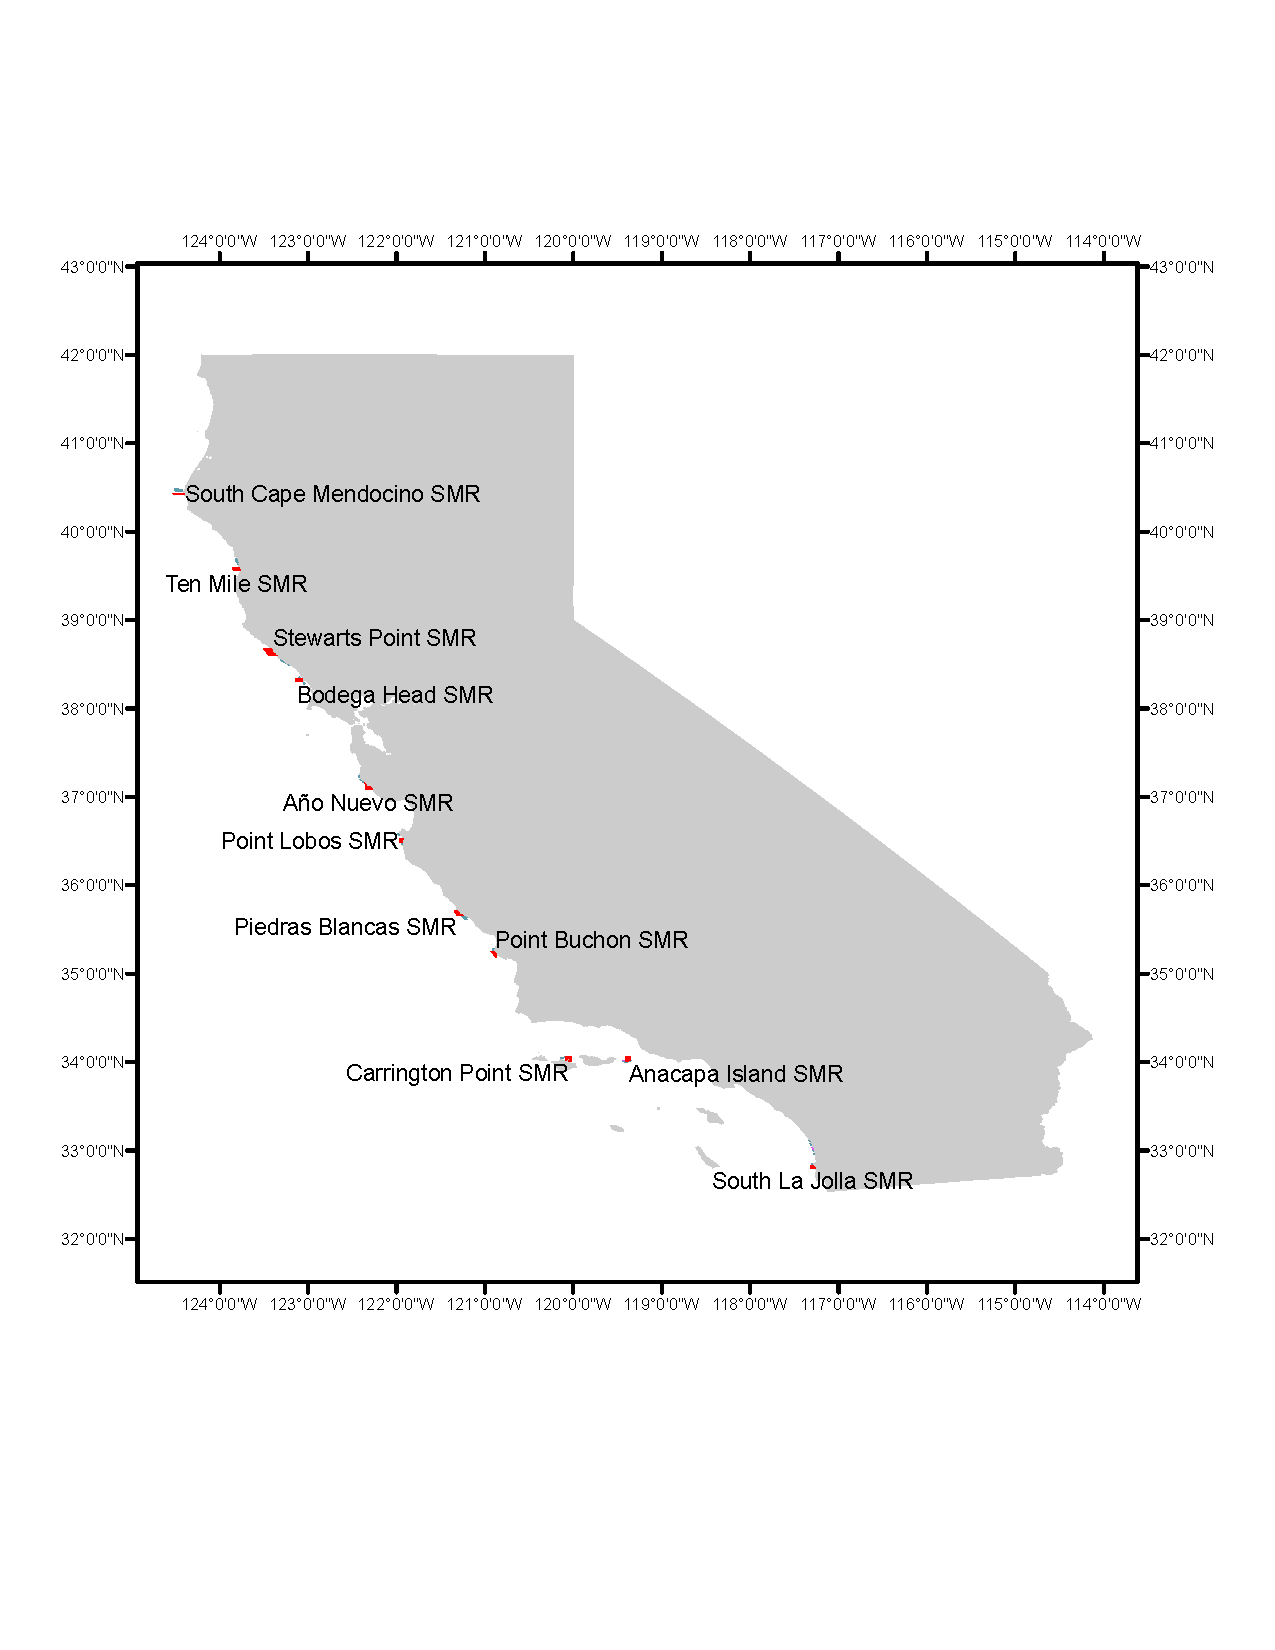
\includegraphics{MPA_map.pdf}
\caption{\label{fig:fig-mpa-map}Map of the State Marine Reserves (SMRs) monitored by the CCFRP program.}
\end{figure}

\begin{figure}
\centering
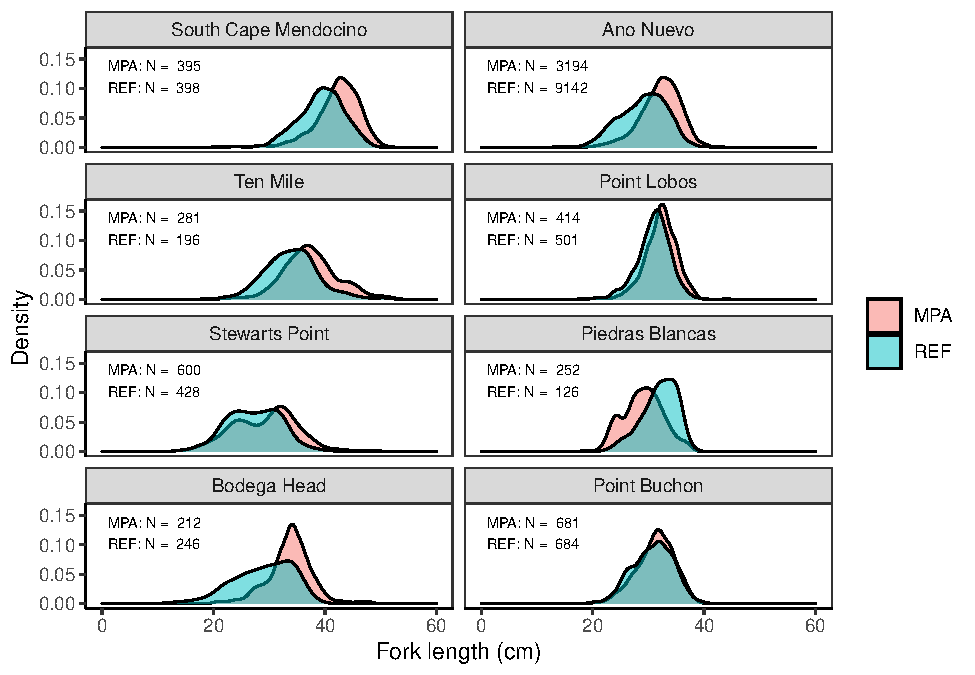
\includegraphics{CCRFP_available_data_for_assessments_files/figure-latex/lengths-1.pdf}
\caption{\label{fig:lengths-1}Density plot of Black Rockfish fork length bins encountered inside each MPA and outside at reference areas (REF) A sample size of NA indicates fewer than 20 fish were encountered in that MPA stratum and were not plotted.}
\end{figure}

\begin{figure}
\centering
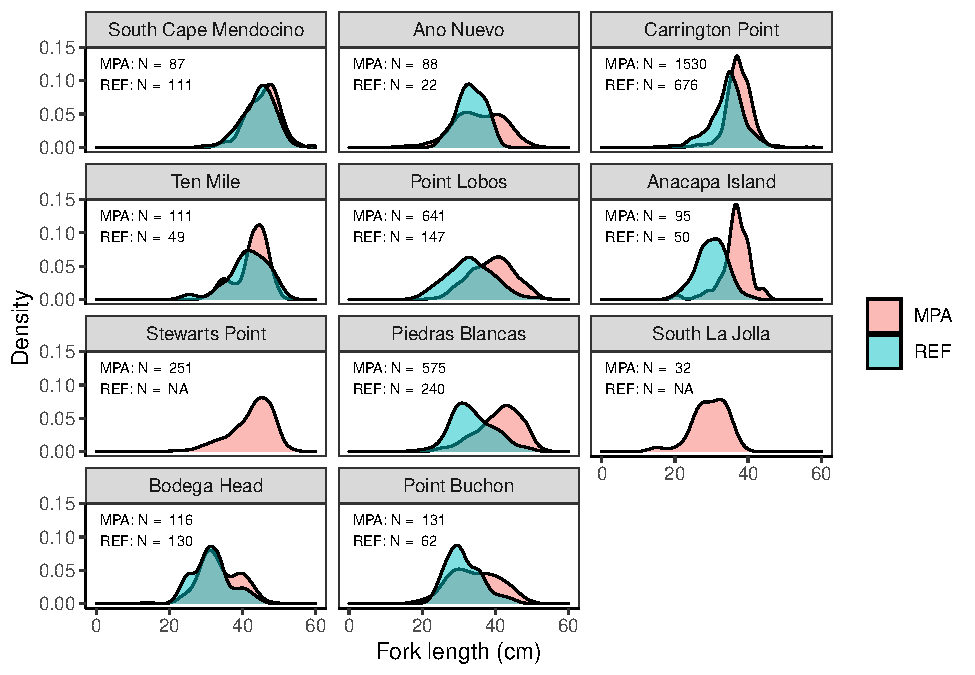
\includegraphics{CCRFP_available_data_for_assessments_files/figure-latex/lengths-2.pdf}
\caption{\label{fig:lengths-2}Density plot of Copper Rockfish fork length bins encountered inside each MPA and outside at reference areas (REF) A sample size of NA indicates fewer than 20 fish were encountered in that MPA stratum and were not plotted.}
\end{figure}

\begin{figure}
\centering
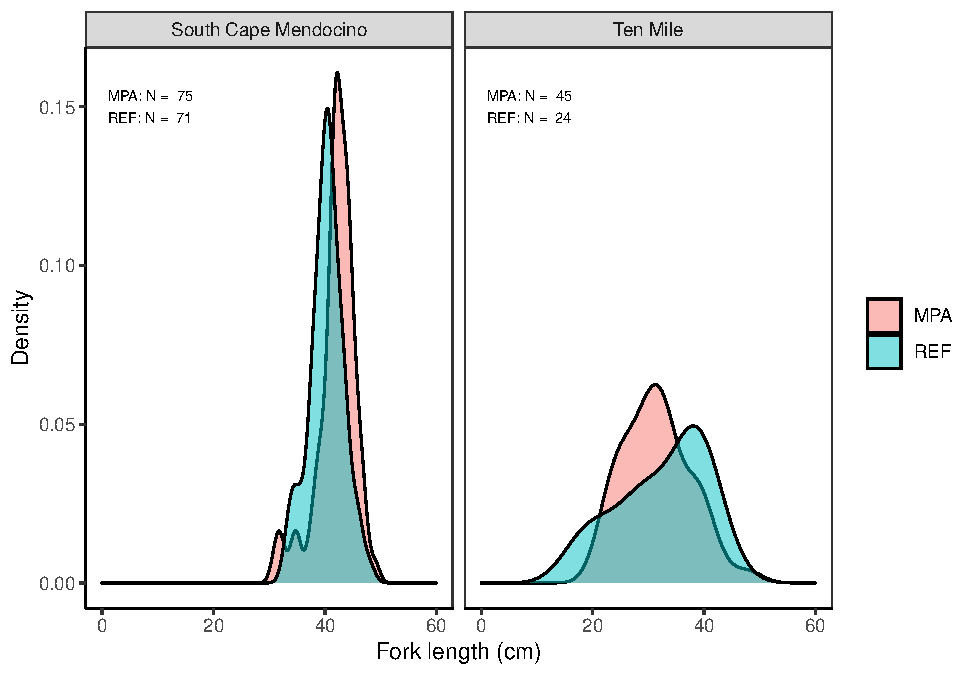
\includegraphics{CCRFP_available_data_for_assessments_files/figure-latex/lengths-3.pdf}
\caption{\label{fig:lengths-3}Density plot of Quillback Rockfish fork length bins encountered inside each MPA and outside at reference areas (REF) A sample size of NA indicates fewer than 20 fish were encountered in that MPA stratum and were not plotted.}
\end{figure}

\begin{figure}
\centering
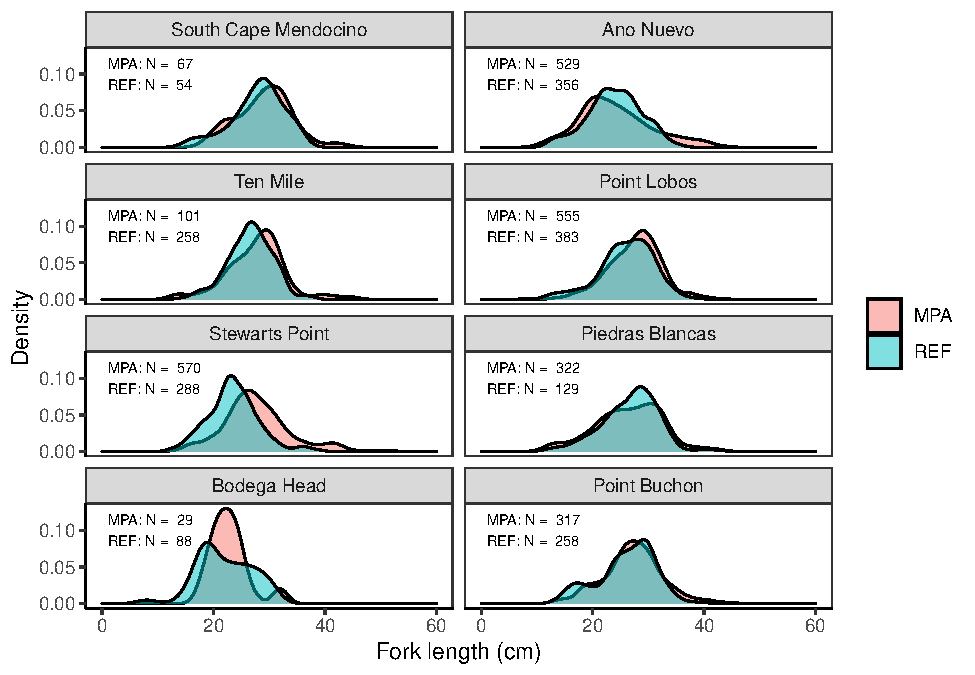
\includegraphics{CCRFP_available_data_for_assessments_files/figure-latex/lengths-4.pdf}
\caption{\label{fig:lengths-4}Density plot of Yellowtail Rockfish fork length bins encountered inside each MPA and outside at reference areas (REF) A sample size of NA indicates fewer than 20 fish were encountered in that MPA stratum and were not plotted.}
\end{figure}

\FloatBarrier

\end{document}
